%fiber_modeling

%\section{Modeling the Lensed Fiber}

Firstly, it is demanded to determine the Tapered and Lensed Fiber(TLF) model. Because of the heave computing cost creating a full size fiber is not economical. Therefore only the end of the fiber, which provides approximately the equal technical properties, will be modeled in this article. In \cite{TLF_analysis} \cite{TLF_mode_transforming} two type of the TLF configuration are mentioned. 


\begin{figure}
\centering
\subfigure[Tapered cladding TLF.]{
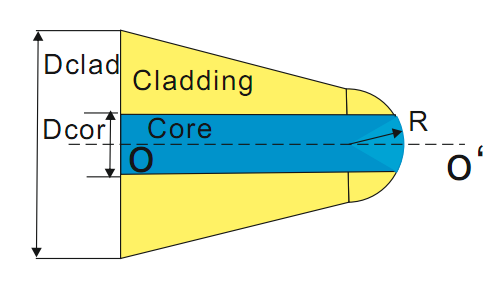
\includegraphics[width=0.4\textwidth]{bilder/lense_fiber_01}
\label{fig:lense_fiber_01}
}
\hfill
\subfigure[Tapered core TLF.]{
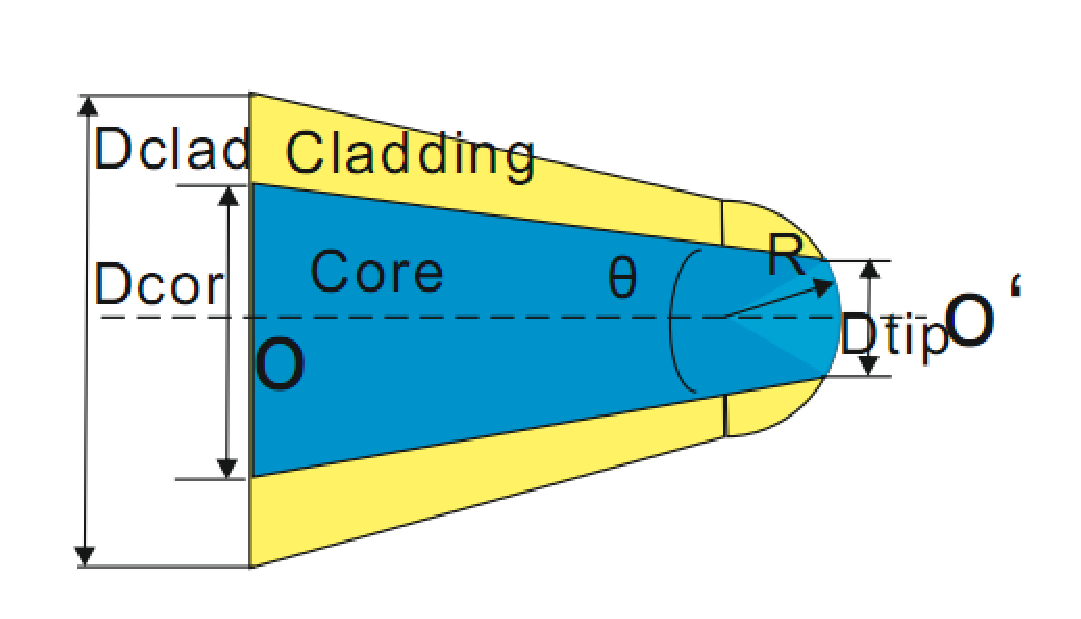
\includegraphics[width=0.4\textwidth]{bilder/lense_fiber_02}
\label{fig:lense_fiber_02}
}
\label{fig:two_TLF}
\caption{Two types of Tapered and Lensed Fibers}
\end{figure}

The Tapered Cladding TLF Fig.\ref{fig:lense_fiber_01} shows that its cladding diameter decreases along the axis and its core diameter is a constant. For the Tapered Core TLF Fig.\ref{fig:lense_fiber_02} its cladding diameter and core diameter both decrease along the axis. In \cite{TLF_mode_transforming} the Authour tried to develop methods to estimate the performance of both type of TLF .  But his results show that the performance of the first type of TLF agrees well with the estimation and that of the second type is unpredictable. 
In this article two TLF models from each type are created and their performances are tested in CST MWS. The following Tab.\ref{tab:model_fiber_configuration} indicates the corresponding configurations.


\begin{table}
\begin{tabular}{ccc}
\hline
							&Tapered Cladding&Tapered Core\\
\hline
$R(\mu m)$ & $6$						 &$6$	\\
refractive indices(core)&$1.68$&$1.66$\\
refractive indices(cladding)&$1.68$&$1.66$\\
$D_{clad}(\mu m)$ &	$17$ &	$17$\\
$D_{core}(\mu m)$ & $10$ &	$17$\\
$D_{tip}(\mu m)$  & --   &	$10$\\
\hline
\end{tabular}
\caption{The Configurations of the TLF Models}
\label{tab:model_fiber_configuration}
\end{table}
%2.20
The fowllowing are the E-Field demonstrations in the xz-plane of both type of TLFs.
\begin{figure}
	\subfigure[E-Field demonstration of Tapered cladding TLF]{
		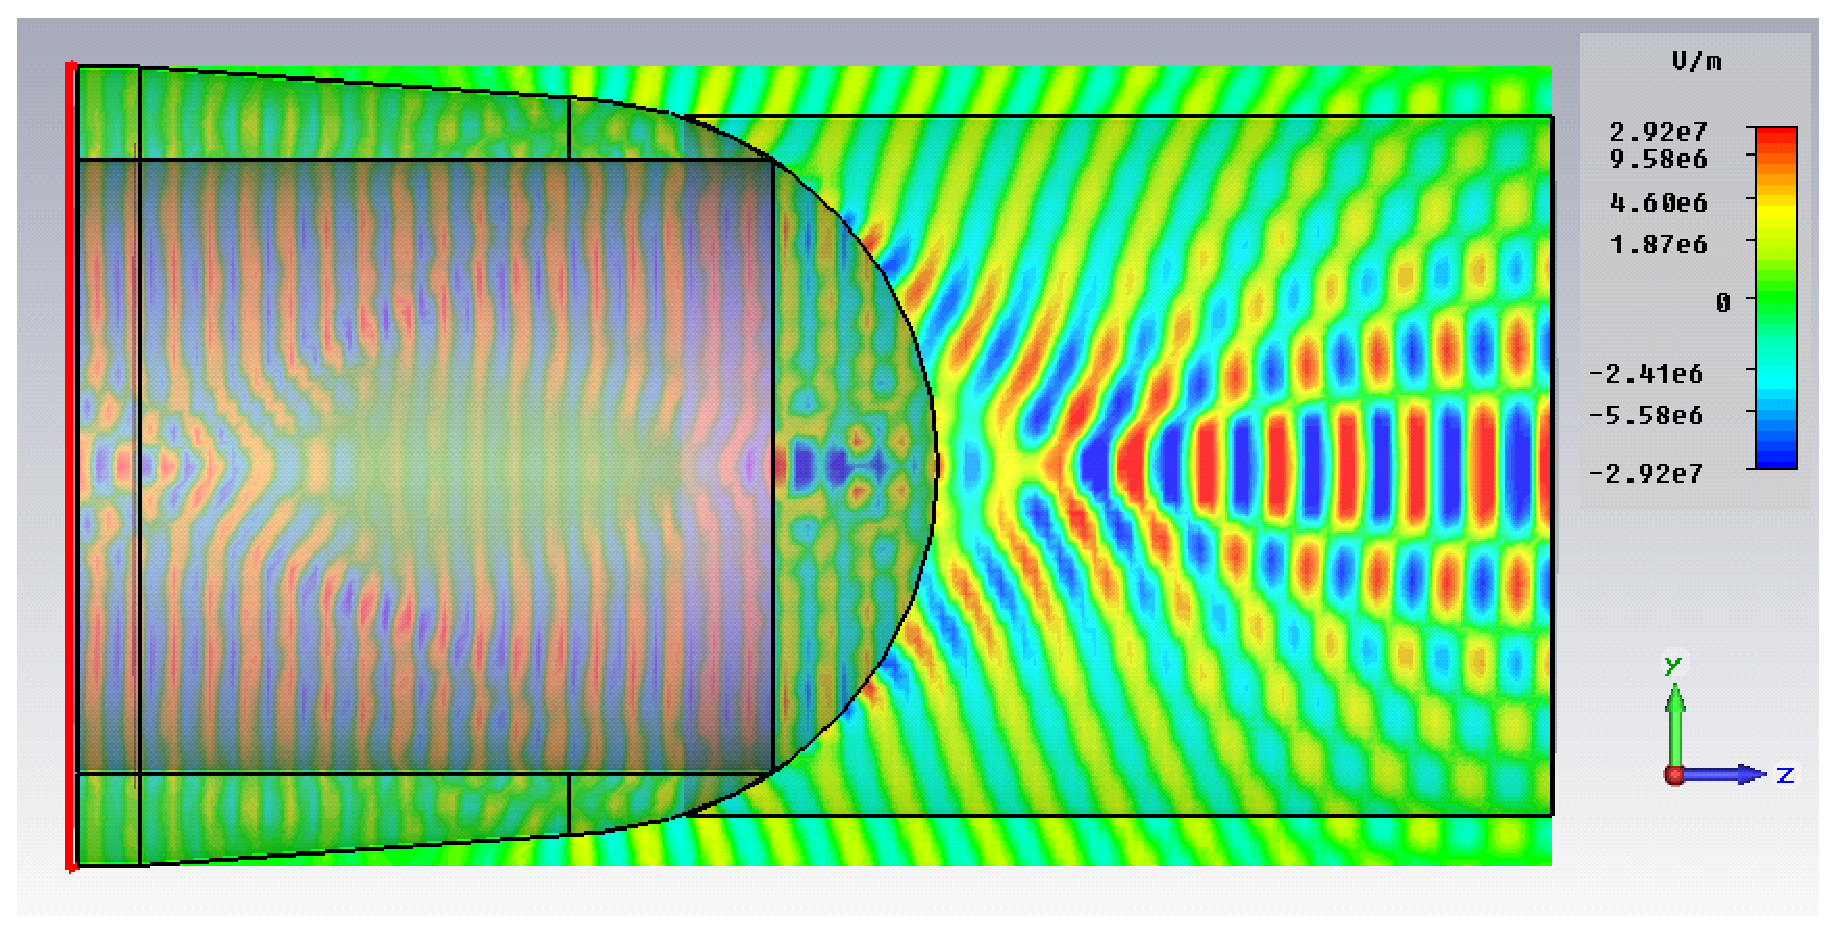
\includegraphics[width=0.4 \textwidth]{bilder/cst_lensed_fiber_equ_efield}
 		\label{fig:Tapered_cladding_efield}
	}
	\hfill
	\subfigure[E-Field demonstration of Tapered core TLF]{
		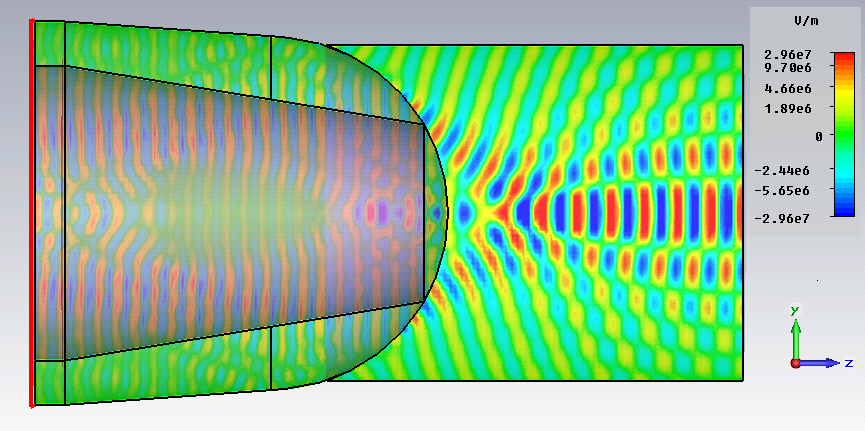
\includegraphics[width=0.4 \textwidth]{bilder/cst_lensed_fiber_efield}
 		\label{fig:Tapered_core_efield}	
	}
	\caption{E Field demonstration}
\end{figure}



As is in section lense theory introduced, the minimum spot located not exactly at the focal length. By using the location of PP and that of MP the MS can be estimated.Fig.\ref{fig:lens_spot} are the theoretical beam propagation of the lense model. The theoretical distance from lens end to PP is $8.82 \mu m$ and the distance from lens end to MP is  $2.74 \mu m$. Backword $3/4$ LAM form PP, the MS is founded at about $4.26 \mu m$far from lens end. 
\begin{figure}
\centering
\subfigure[complete Beam Propogation from lense.]{
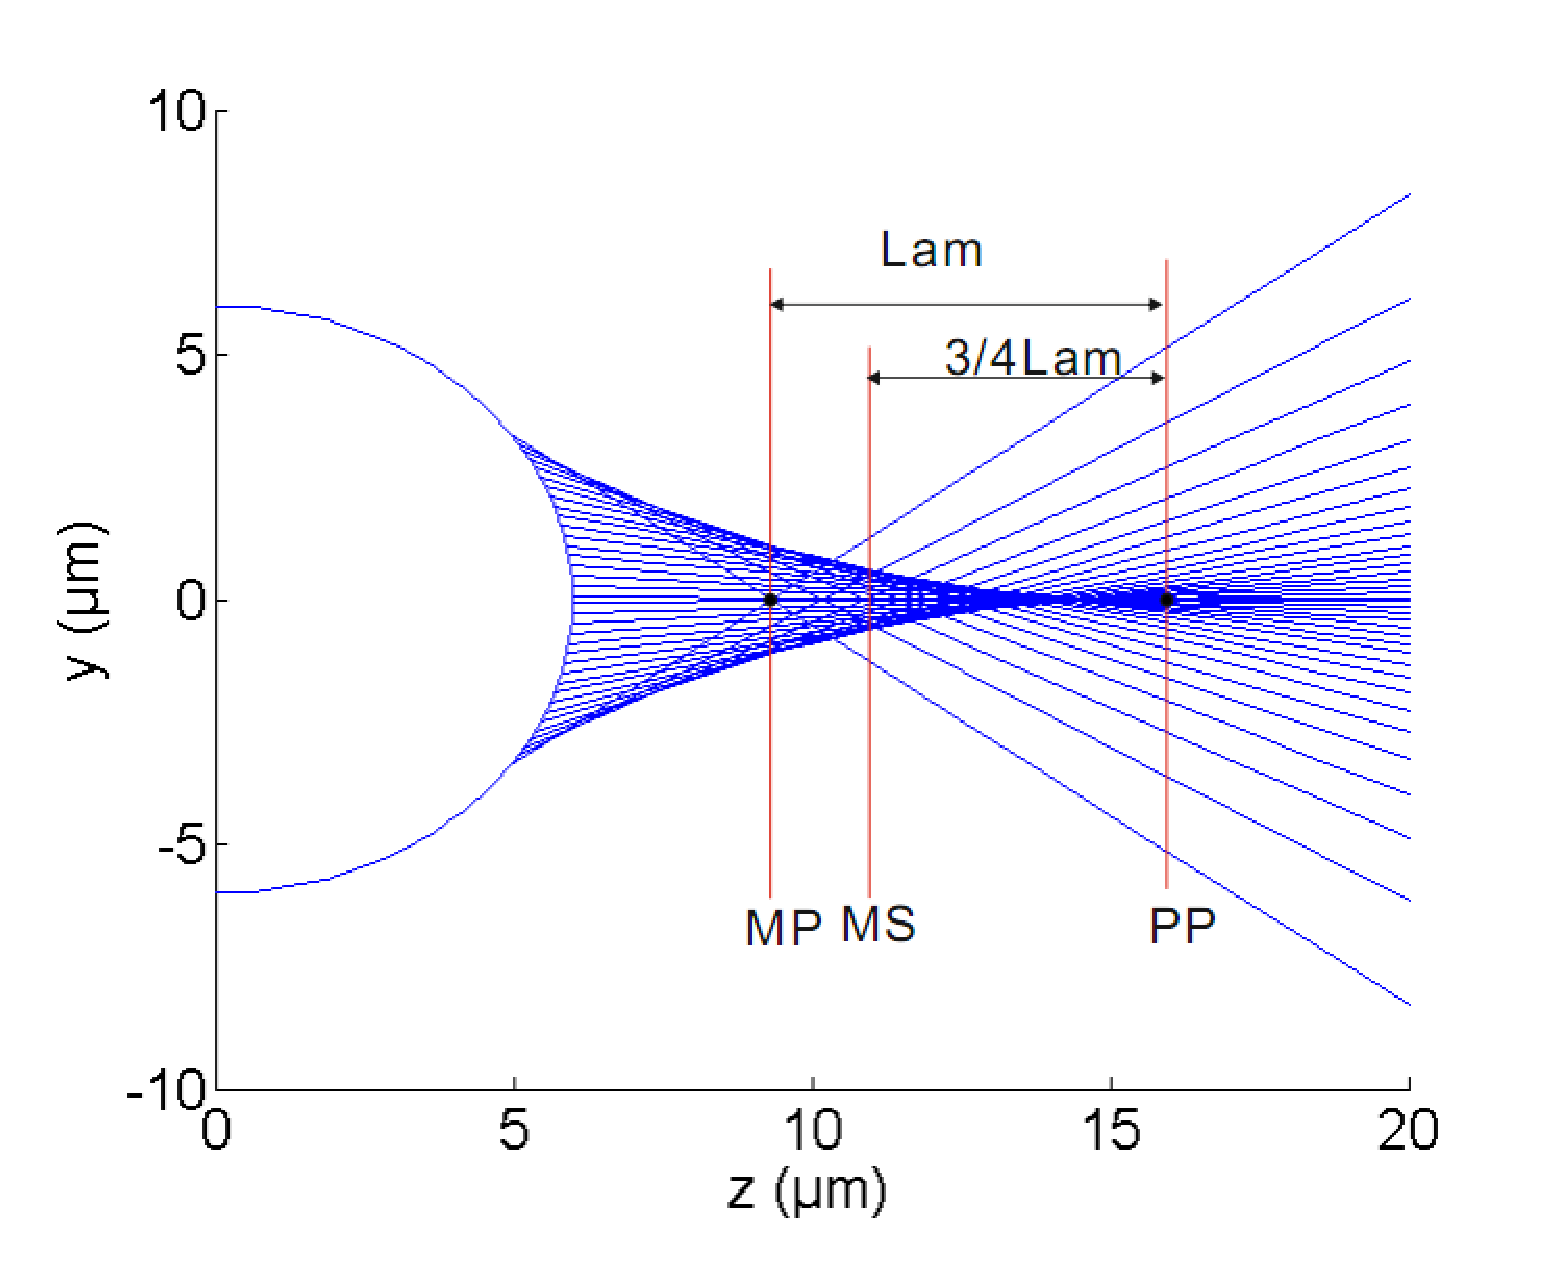
\includegraphics[width=0.4\textwidth]{bilder/cal_min_spot}
\label{fig:lense_cal_spot1}
}
\hfill
\subfigure[half Beam Propogation from lense and calculating the minimue spot.]{
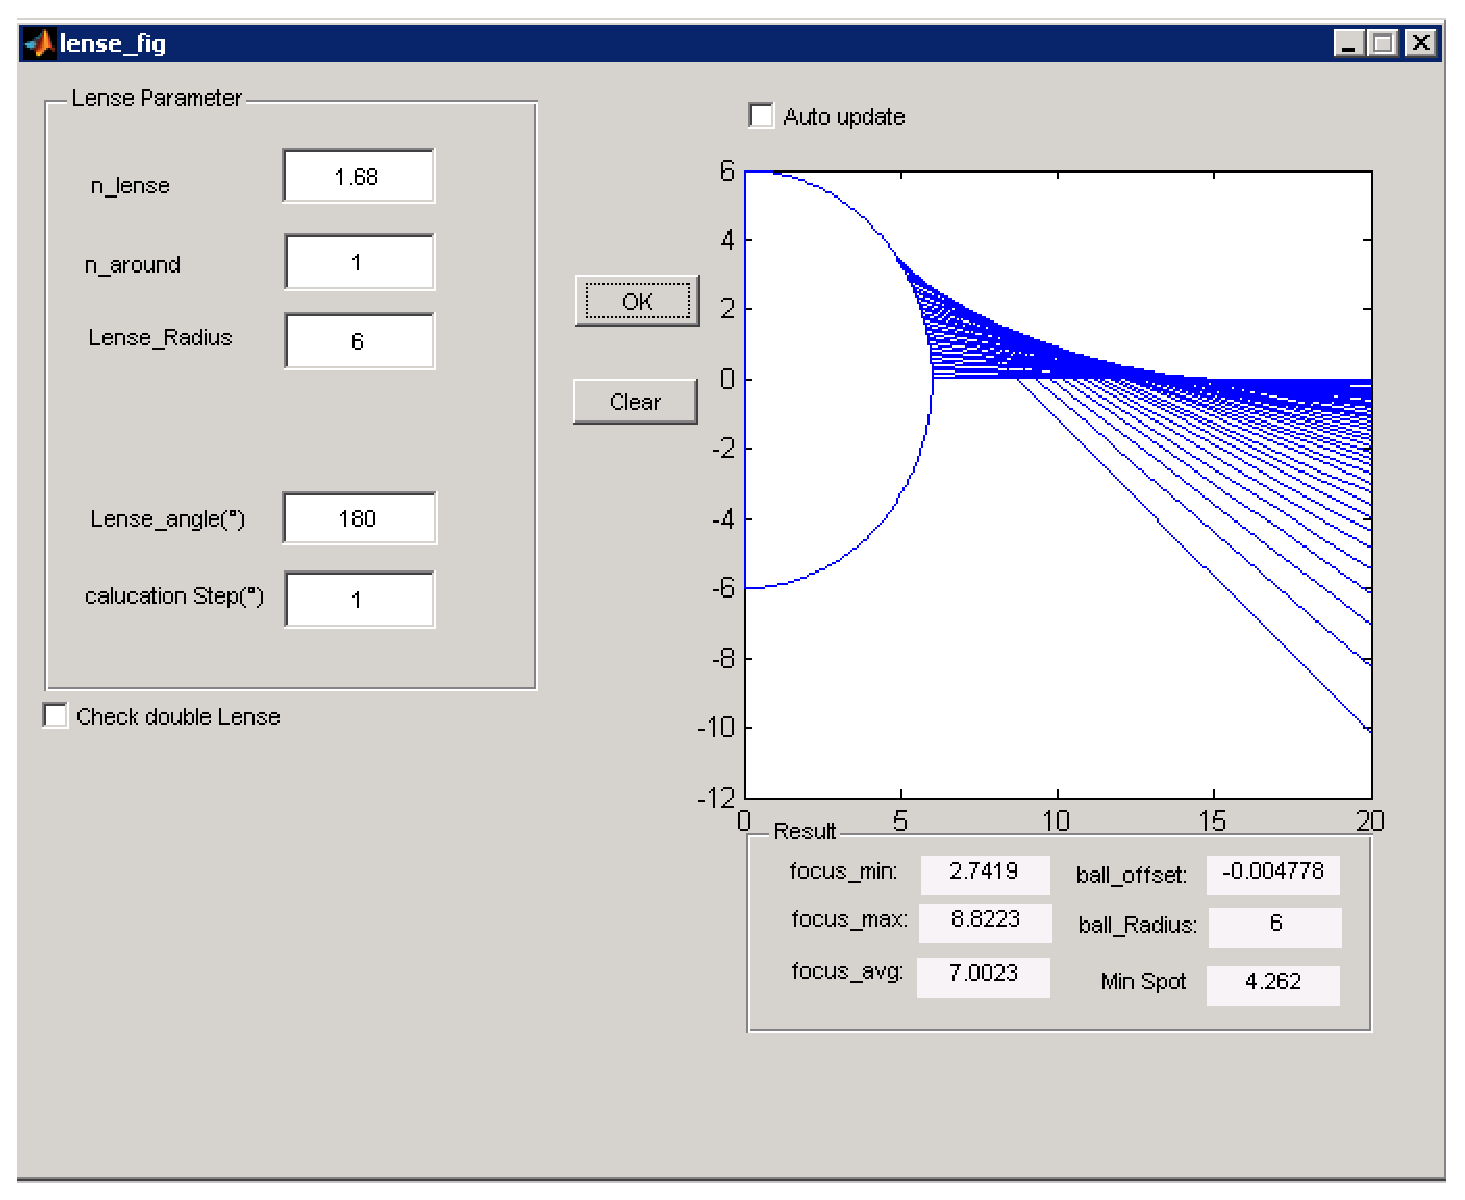
\includegraphics[width=0.4\textwidth]{bilder/lens_cal_spot_168}
\label{fig:lense_cal_spot2}
}
\label{fig:lens_spot}
\caption{calculating minimus spot size by lense theory.}
\end{figure}
Load the its beam propagation detail into \textbf{Matlab} workspace and check the 2D and 3D beam power distribution in different distance. Fig.(\ref{fig:2d_spot_sub1}-\ref{fig:2d_spot_sub8}) and Fig.(\ref{fig:3d_spot_sub1}-\ref{fig:3d_spot_sub8}) respectively.%2D and 3D
\begin{figure}
\setlength{\abovecaptionskip}{0pt}% 
\flushleft
	\subfigure[2D Beam Power at distance $1\mu m$]{
	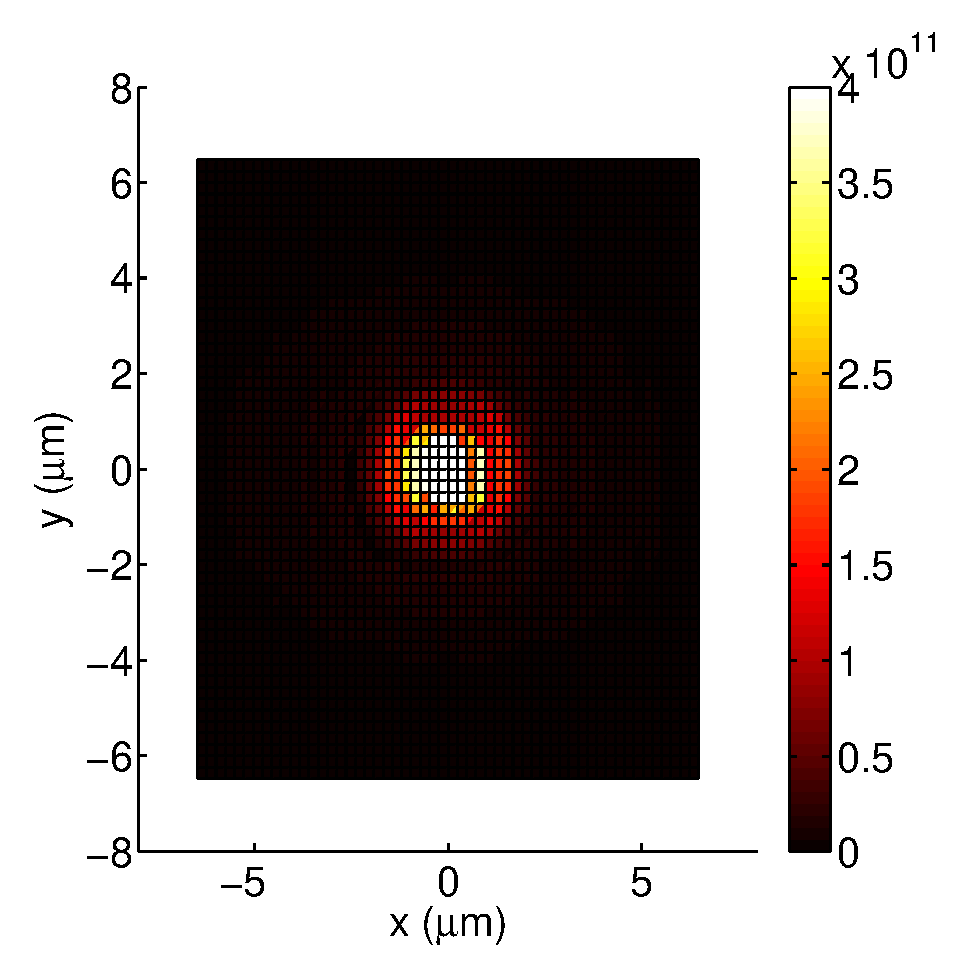
\includegraphics[width=0.29 \textwidth]{bilder/surface_spot_1um}
	\label{fig:2d_spot_sub1}%
	}
 	\subfigure[2D Beam Power at distance $2\mu m$]{
 	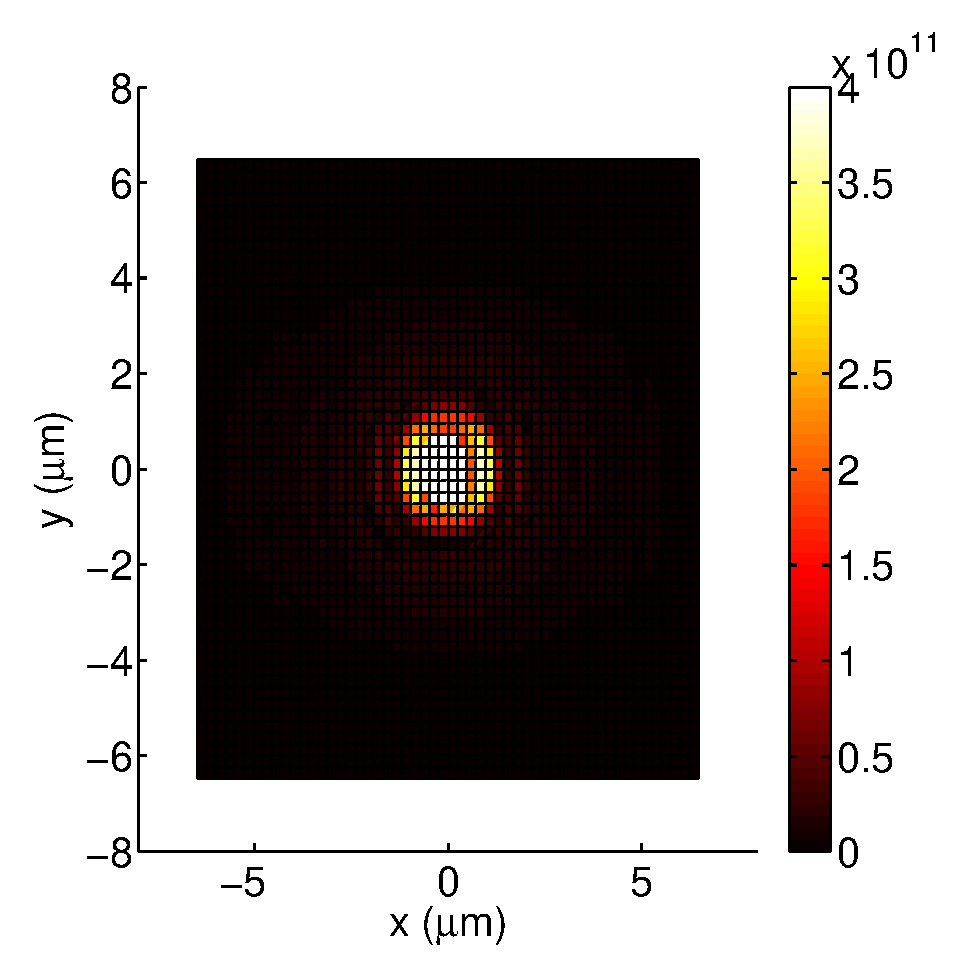
\includegraphics[width=0.29 \textwidth]{bilder/surface_spot_2um}
 	\label{fig:2d_spot_sub2}
 	}
 	 	\subfigure[2D Beam Power at distance $3\mu m$]{
 	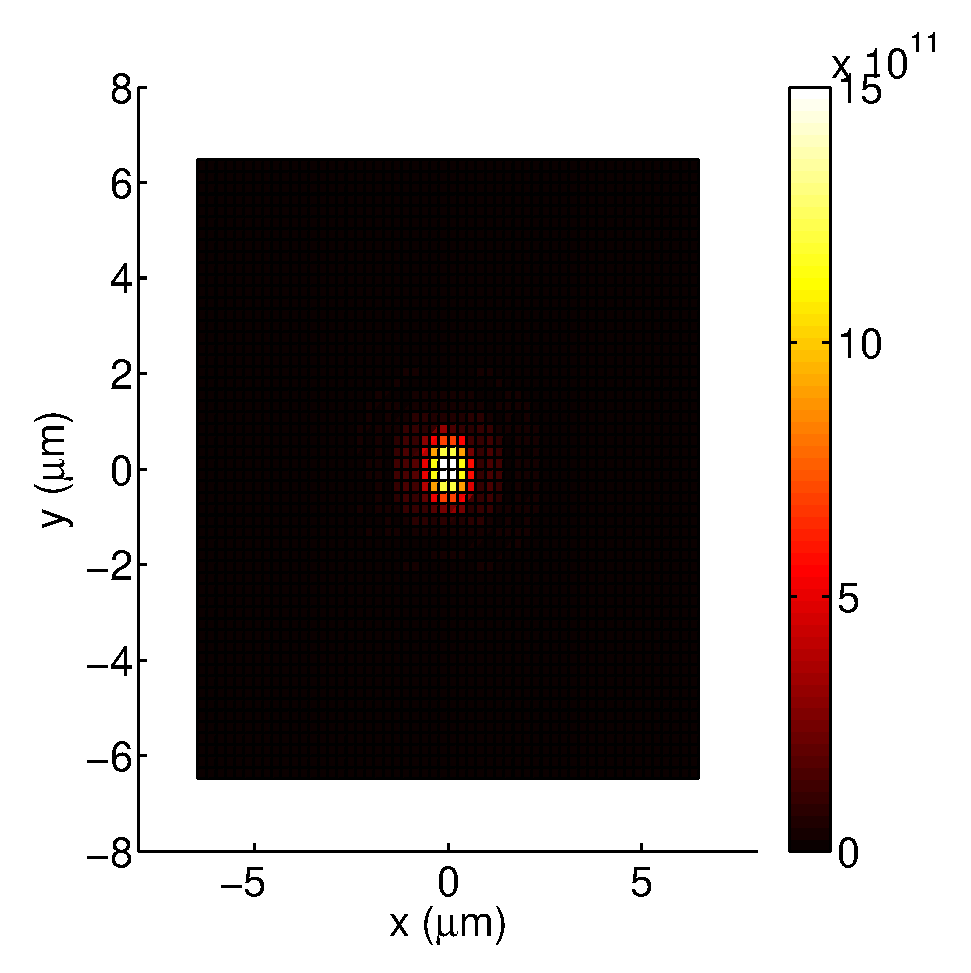
\includegraphics[width=0.29 \textwidth]{bilder/surface_spot_3um}
 	\label{fig:2d_spot_sub3}
 	}
 	\subfigure[2D Beam Power at distance $4\mu m$]{
 	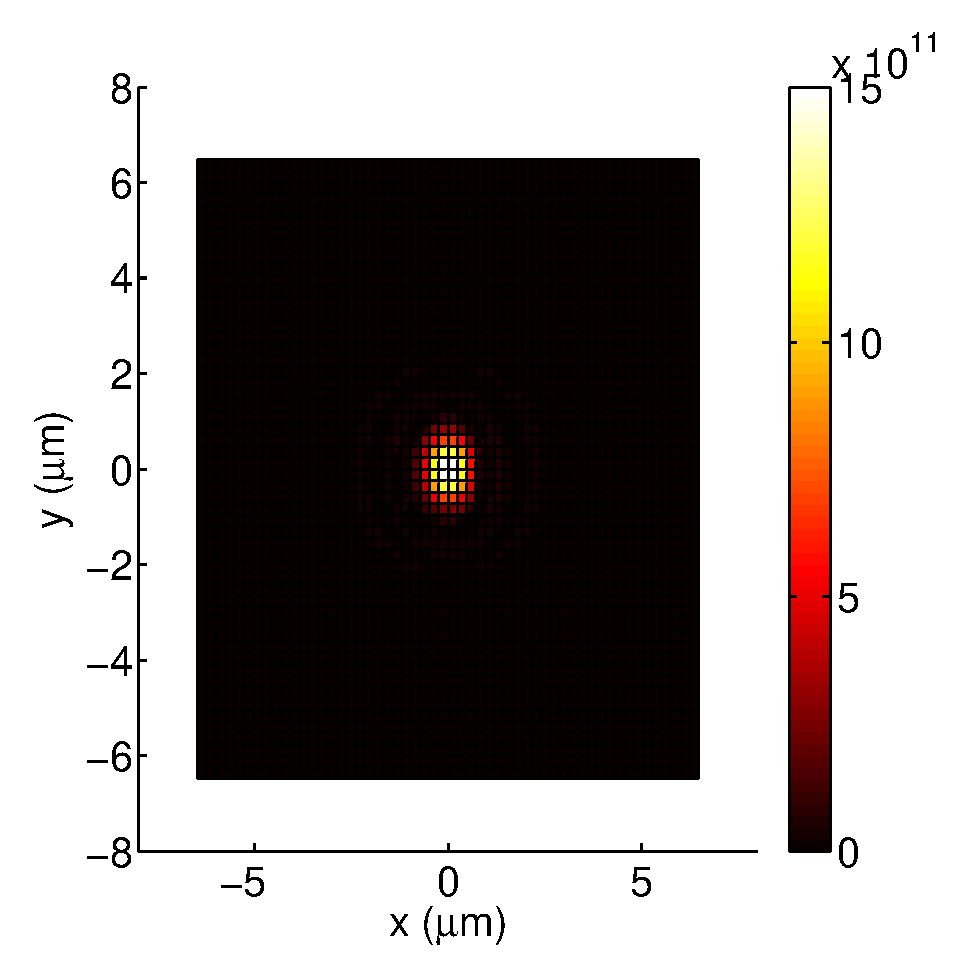
\includegraphics[width=0.29 \textwidth]{bilder/surface_spot_4um}
 	\label{fig:2d_spot_sub4}
 	}
 	 \subfigure[2D Beam Power at distance $5\mu m$]{
 	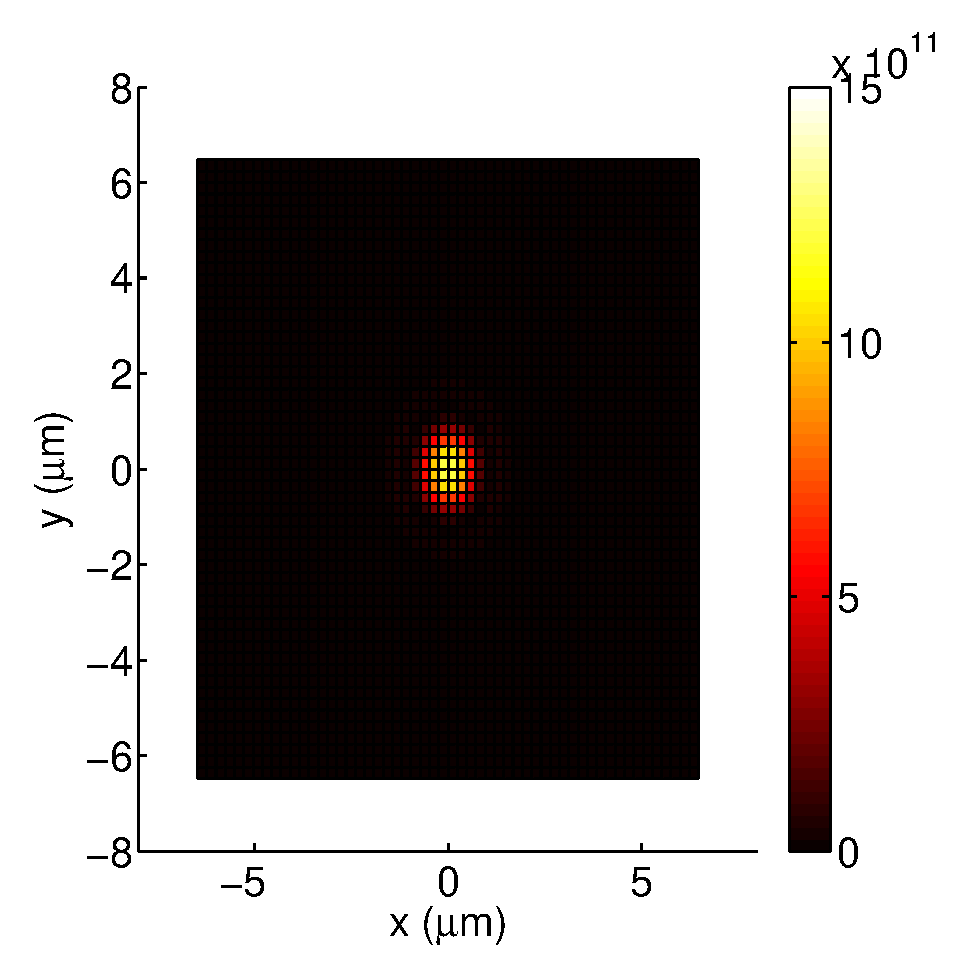
\includegraphics[width=0.29 \textwidth]{bilder/surface_spot_5um}
 	\label{fig:2d_spot_sub5}
 	}
 	 	\subfigure[2D Beam Power at distance $6\mu m$]{
 	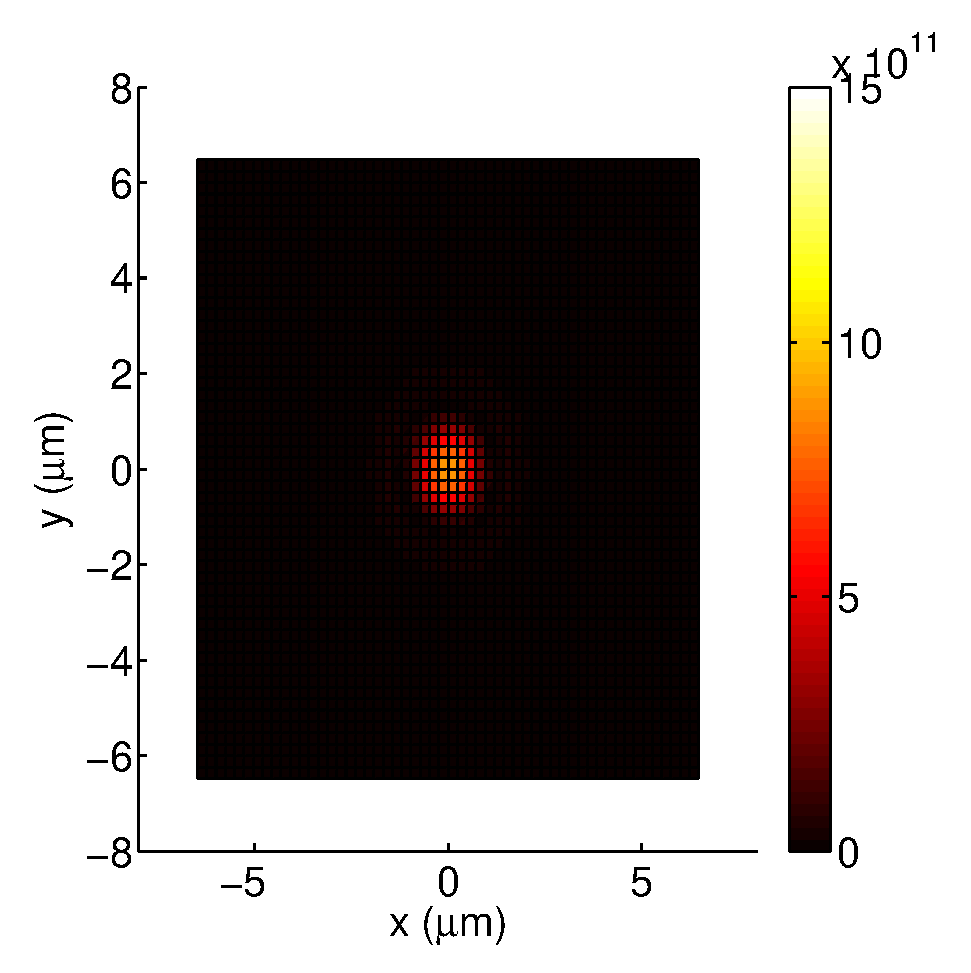
\includegraphics[width=0.29 \textwidth]{bilder/surface_spot_6um}
 	\label{fig:2d_spot_sub6}
 	}
  \subfigure[2D Beam Power at distance $7\mu m$]{
 	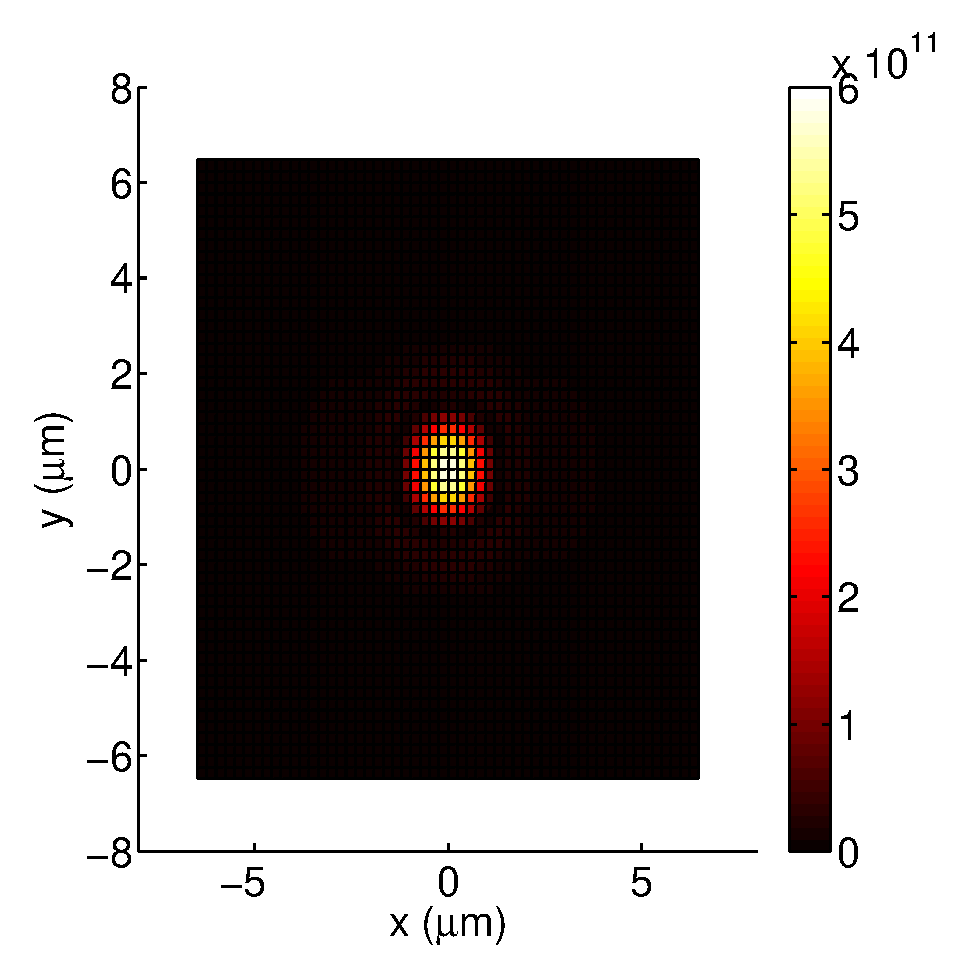
\includegraphics[width=0.29 \textwidth]{bilder/surface_spot_7um}
 	\label{fig:2d_spot_sub7}
 	}
 	\subfigure[2D Beam Power at distance $8\mu m$]{
 	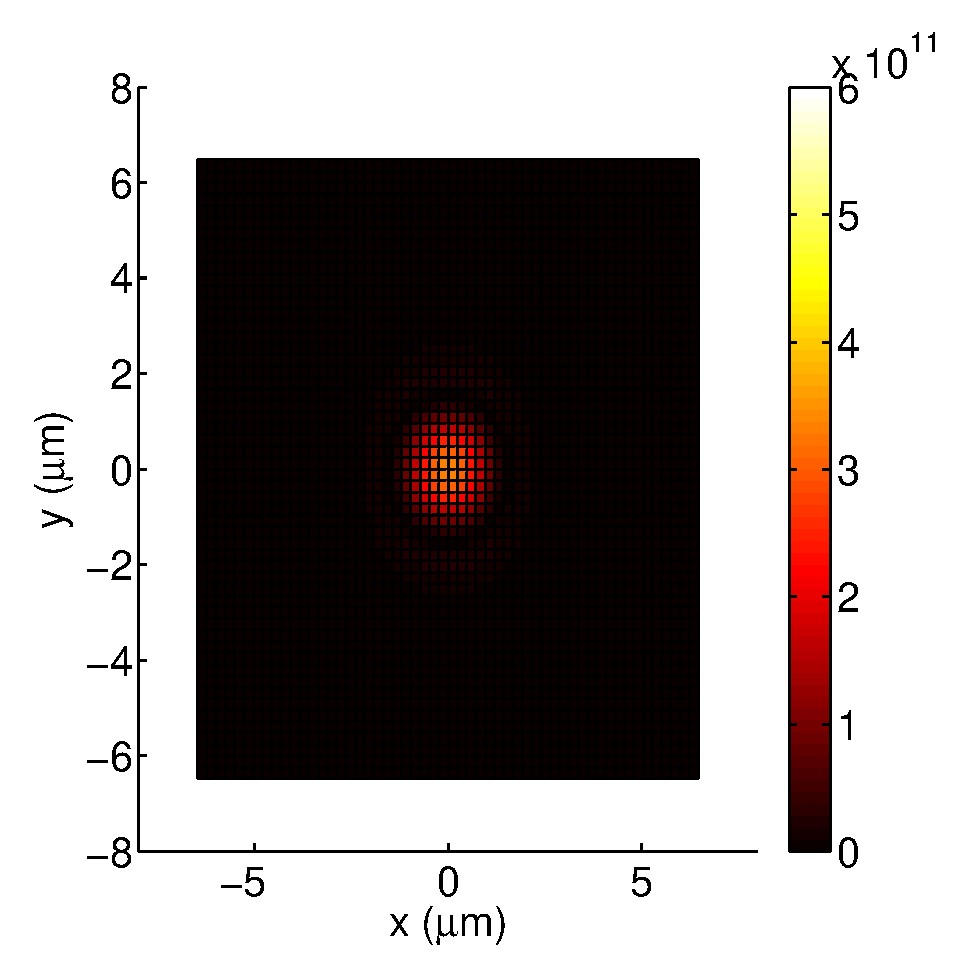
\includegraphics[width=0.29 \textwidth]{bilder/surface_spot_8um}
 	\label{fig:2d_spot_sub8}
 	}
 	\caption{2D Beam Spot }
\end{figure}

\begin{figure}
\setlength{\abovecaptionskip}{0pt}% 
\flushleft
	\subfigure[3D Beam Power at distance $1\mu m$]{
	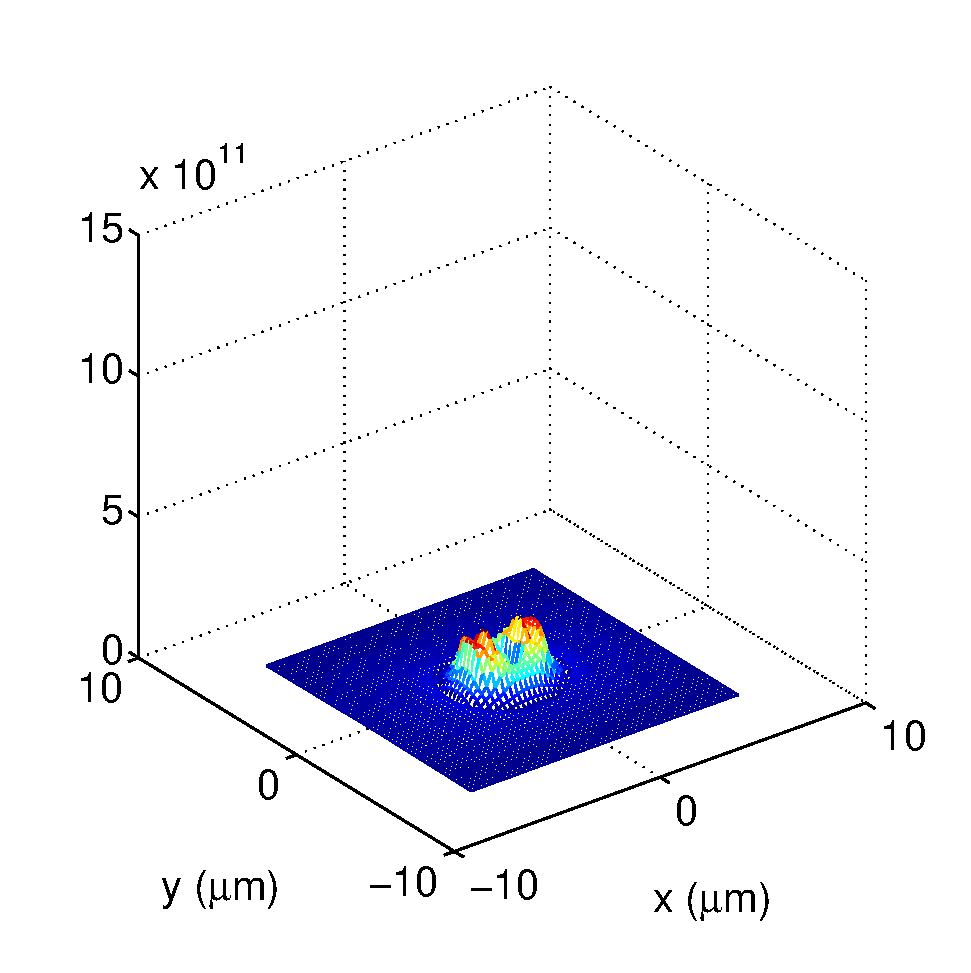
\includegraphics[width=0.26 \textwidth]{bilder/surf_spot_1um}
	\label{fig:3d_spot_sub1}%
	}
 	\subfigure[3D Beam Power at distance $2\mu m$]{
 	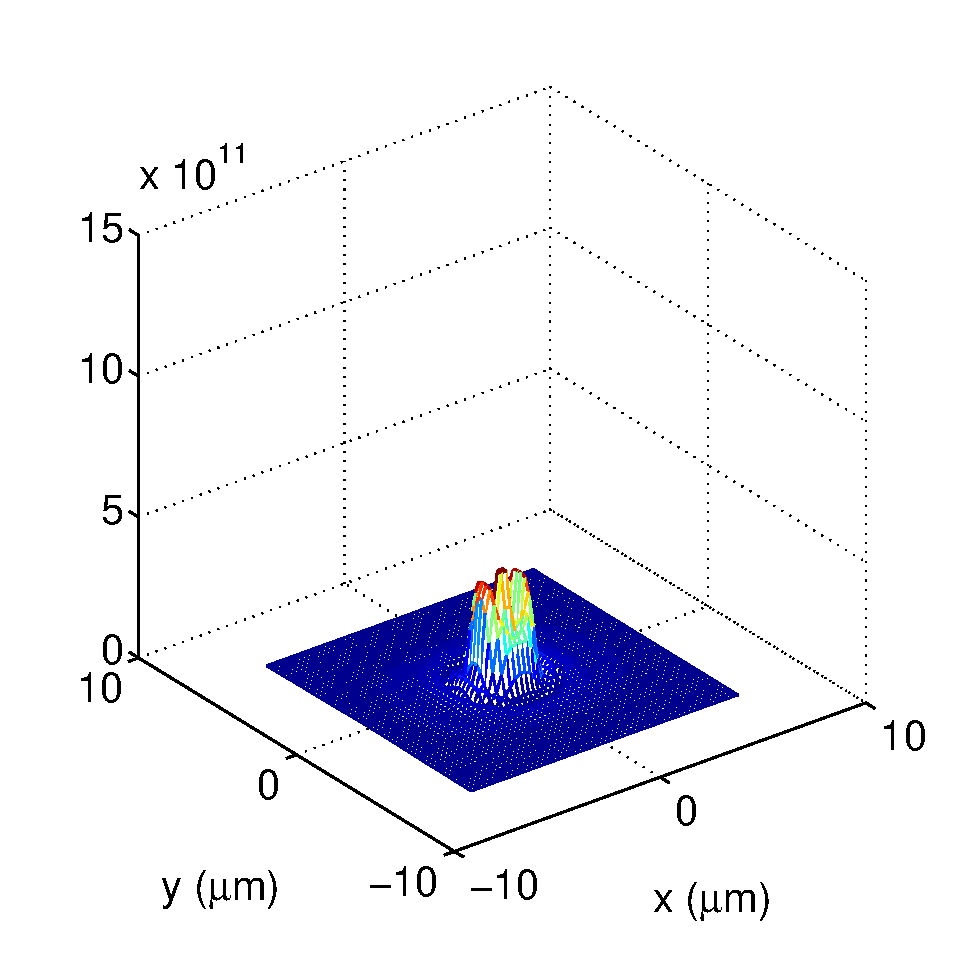
\includegraphics[width=0.26 \textwidth]{bilder/surf_spot_2um}
 	\label{fig:3d_spot_sub2}
 	}
 	 	\subfigure[3D Beam Power at distance $3\mu m$]{
 	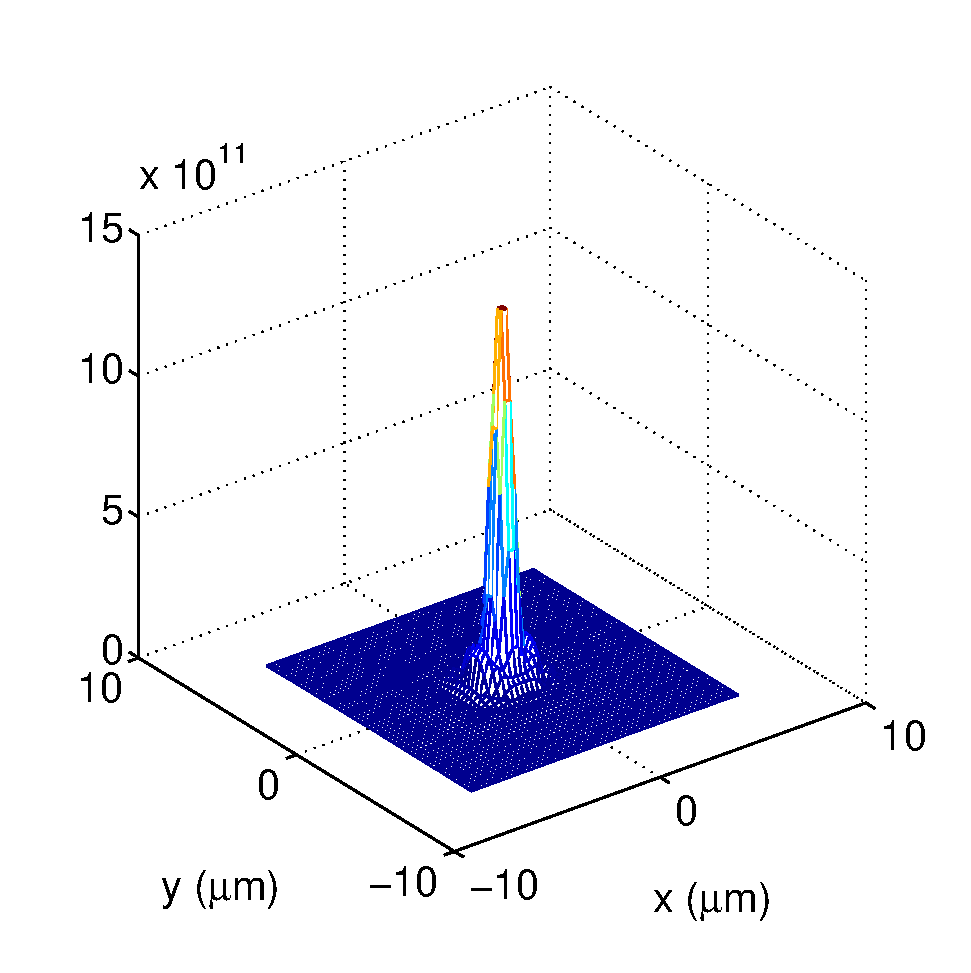
\includegraphics[width=0.26 \textwidth]{bilder/surf_spot_3um}
 	\label{fig:3d_spot_sub3}
 	}
 	\subfigure[3D Beam Power at distance $4\mu m$]{
 	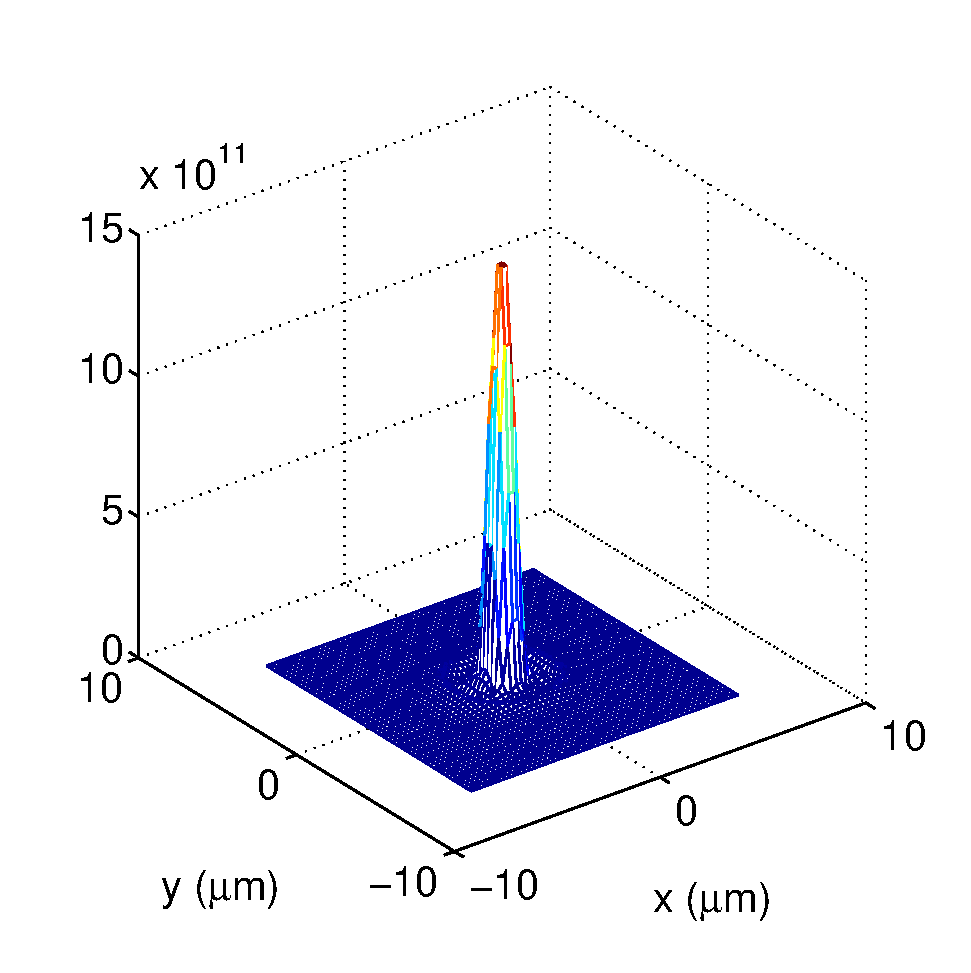
\includegraphics[width=0.26 \textwidth]{bilder/surf_spot_4um}
 	\label{fig:3d_spot_sub4}
 	}
 	 \subfigure[3D Beam Power at distance $5\mu m$]{
 	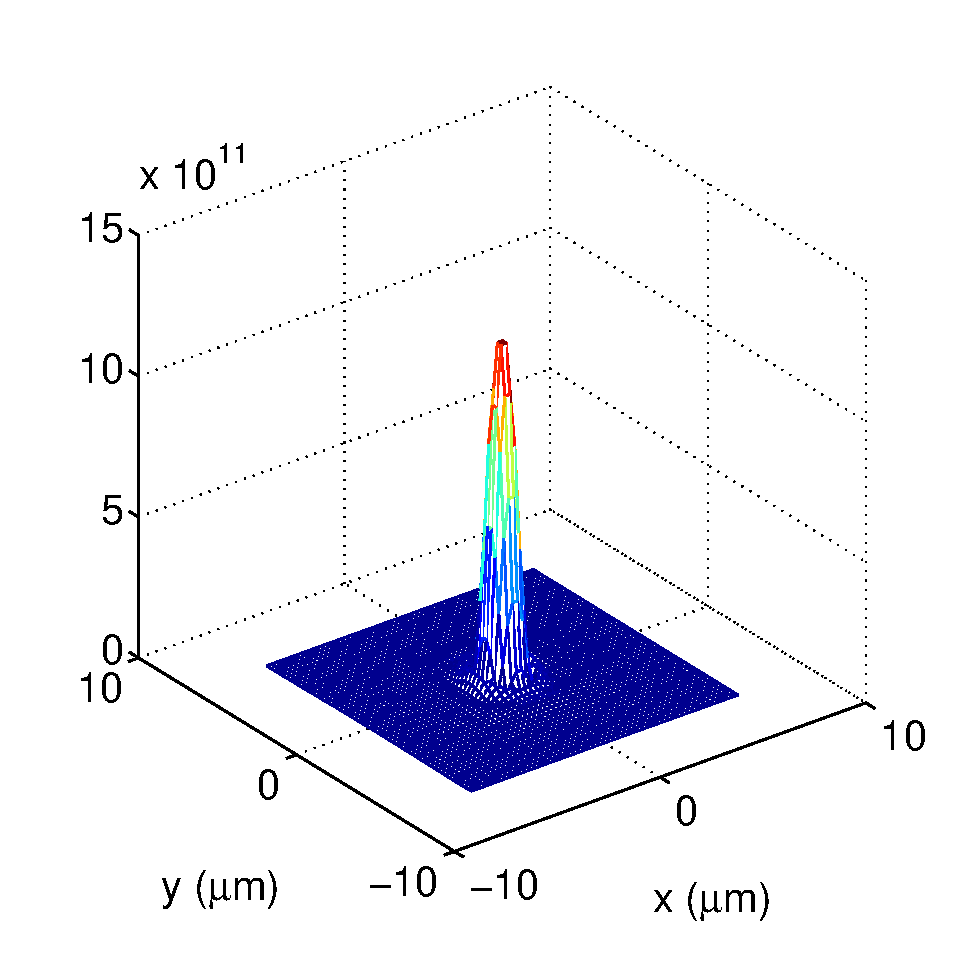
\includegraphics[width=0.26 \textwidth]{bilder/surf_spot_5um}
 	\label{fig:3d_spot_sub5}
 	}
 	 	\subfigure[3D Beam Power at distance $6\mu m$]{
 	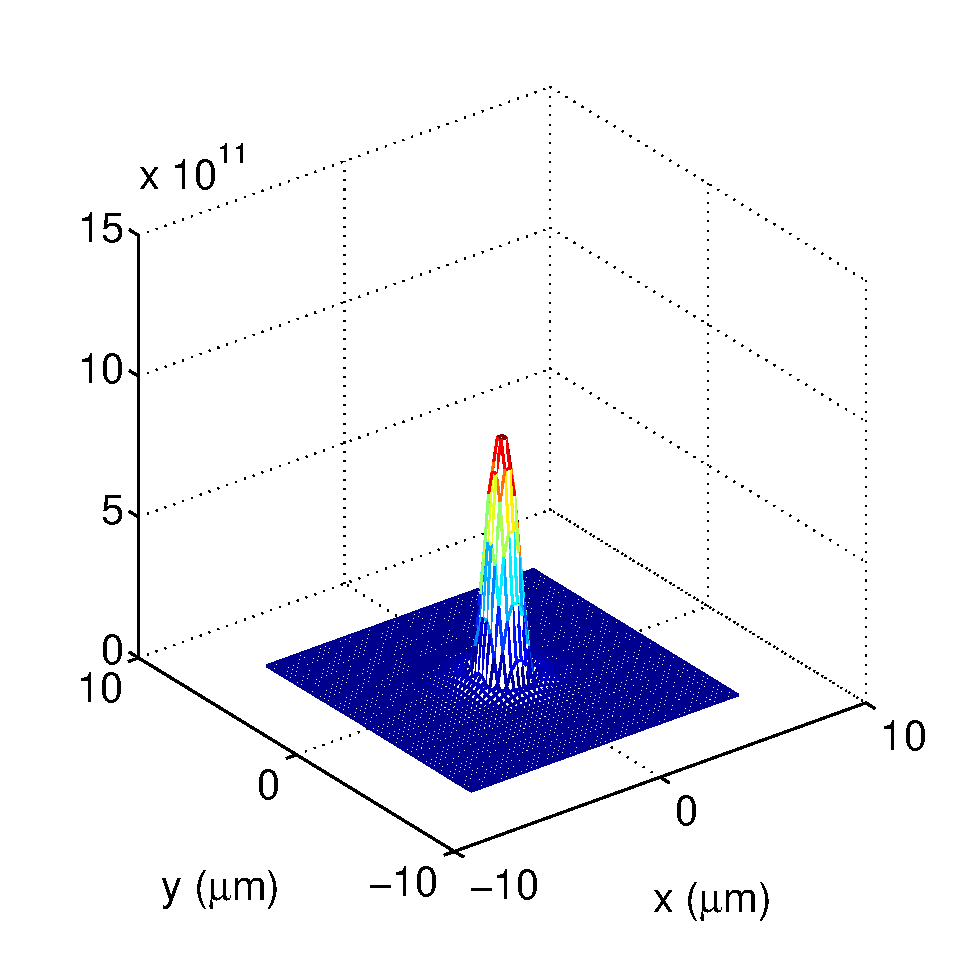
\includegraphics[width=0.26 \textwidth]{bilder/surf_spot_6um}
 	\label{fig:3d_spot_sub6}
 	}
  \subfigure[3D Beam Power at distance $7\mu m$]{
 	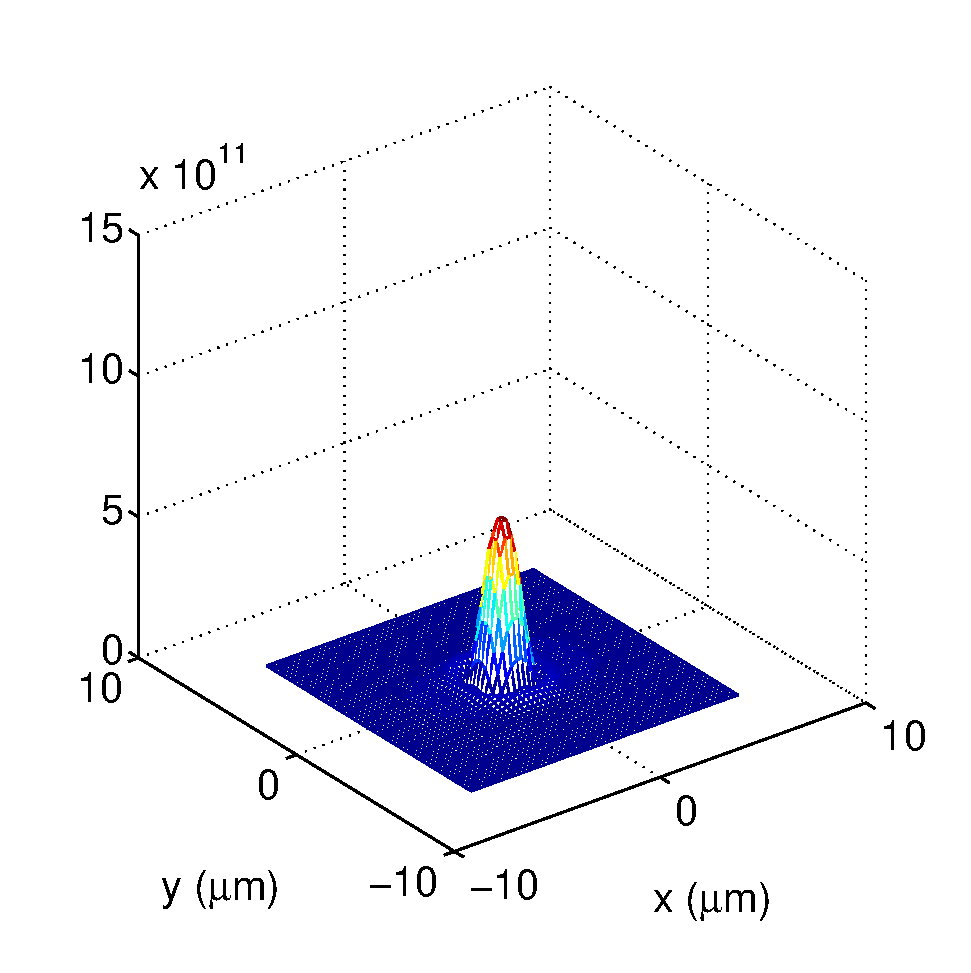
\includegraphics[width=0.26 \textwidth]{bilder/surf_spot_7um}
 	\label{fig:3d_spot_sub7}
 	}
 	\subfigure[3D Beam Power at distance $8\mu m$]{
 	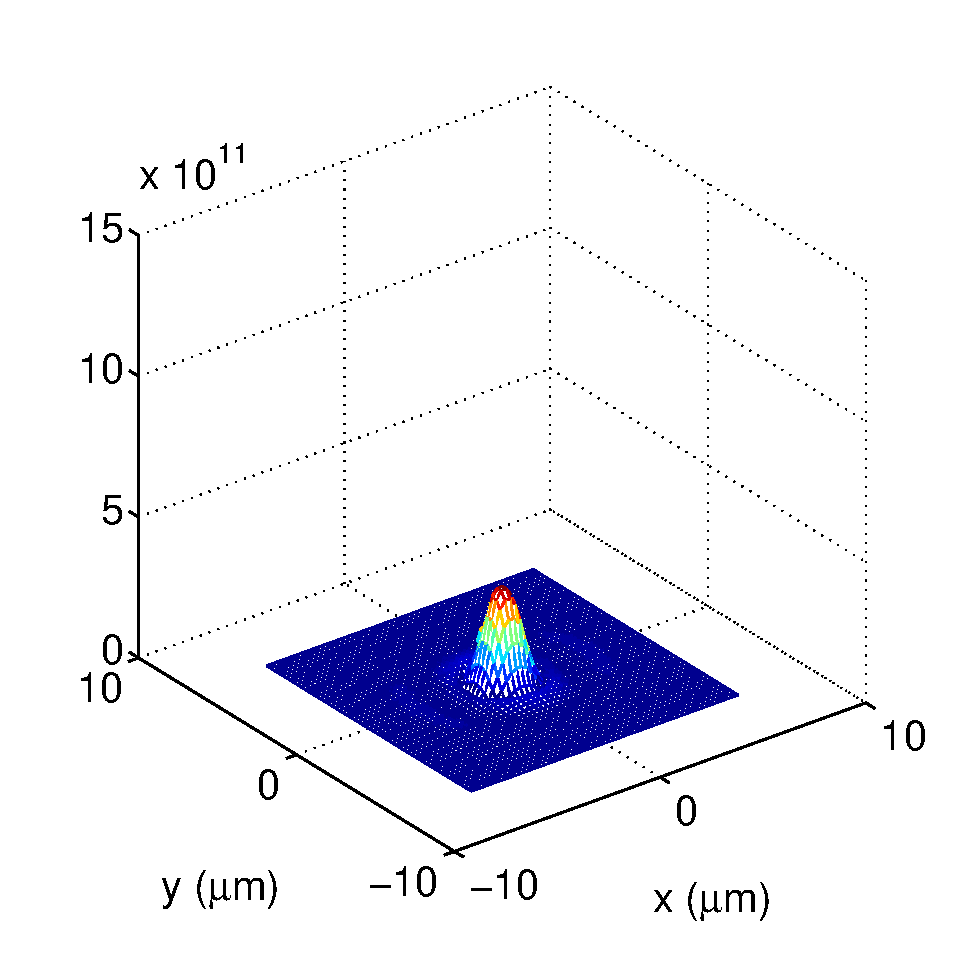
\includegraphics[width=0.26 \textwidth]{bilder/surf_spot_8um}
 	\label{fig:3d_spot_sub8}
 	}
 	\caption{3D Beam Power }
\end{figure} 
Draw Fig.\ref{fig:Tapered_cladding_spot_curve}-\ref{fig:Tapered_core_spot_curve} to illustrate the beam Spot size diameter along the longitude axis.
\begin{figure}
	\subfigure[Spot Size Curve of Tapered cladding TLF]{
		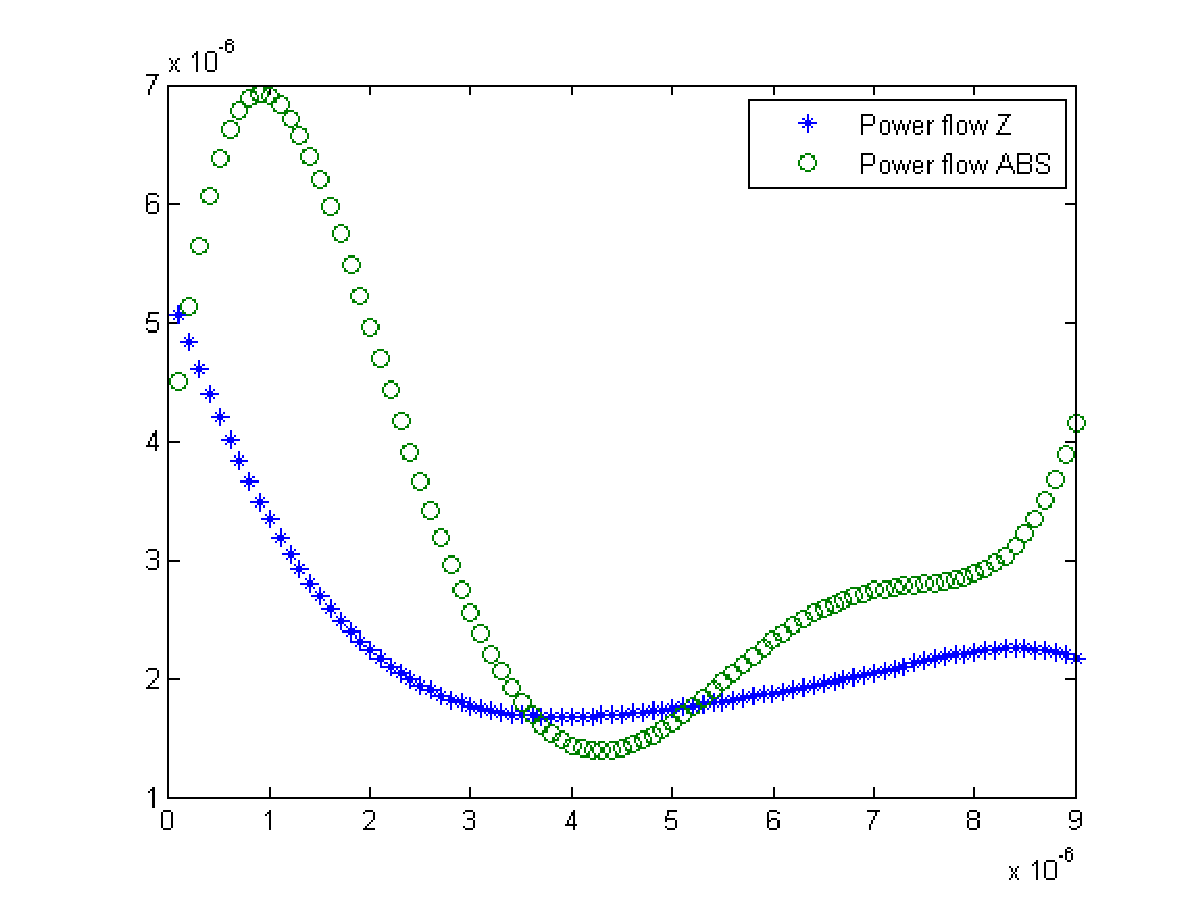
\includegraphics[width=0.4 \textwidth]{bilder/flower_hiber_cladding}
 		\label{fig:Tapered_cladding_spot_curve}
	}
	\hfill
	\subfigure[Spot Size Curve of Tapered core TLF]{
		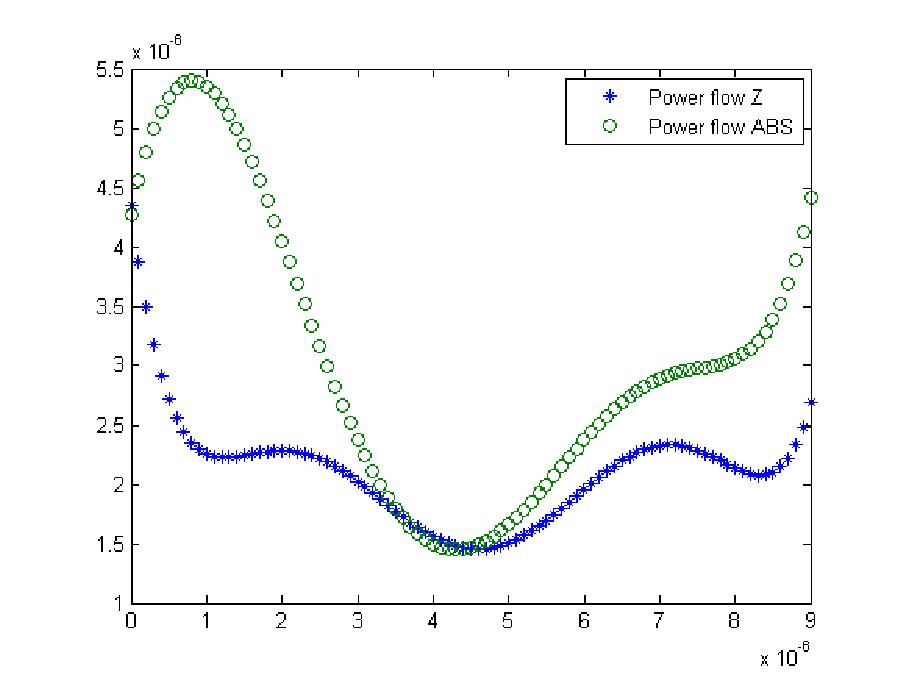
\includegraphics[width=0.4 \textwidth]{bilder/flower_hiber_core}
 		\label{fig:Tapered_core_spot_curve}	
	}
\caption{Curve of Spot size diameter}
\end{figure}
Fig.\ref{fig:Tapered_cladding_spot_curve} and Fig.\ref{fig:Tapered_core_spot_curve} shows the spot diameters of both configurrations along the propogation direction by using z-compent and absolute value of their power flow density. Here choose the curve from absolute value of their power flow density to determine the minimum spot. From Fig.\ref{fig:Tapered_cladding_spot_curve} that the minimum spot size locate at about $4.1 \mu m$ from lense end and spot size equal about $1.5 \mu m$. While in Fig.\ref{fig:Tapered_core_spot_curve} that the minimum spot size is found at  $4.3 \mu m$ from lense end and spot size equal about $1.5 \mu m$. Thus it is concluded that two configuration has only a small difference. By rechecking the properties in Tab.\ref{tab:technical parameters_lensed_fiber} both TLF model are acceptable for the following development. In this article the Tapered core TLF will be used for further simulations. 
